\newpage \section{Backgrounds}
\label{sec:bkg}
(background in vdM, afterglow backgrounds in Physics, subtraction of these) \\

N= \sigma \:L + N_{background} \\

L = $ \int L_{inst} \: dt = \int \frac{R(t)}{\sigma_{vis}} \:dt $  \\

\sigma = \sigma_{interaction} (\sqrt{s}) \: A \:\epsilon\\

N: total number of event including signal and background. \\

$R(t) = \frac{d}{dt} <N_{cluster}>$ is the time dependent cluster rate. \\

$N_{background}$: Number of background events \\

$\sigma_{vis}$: PCC visible cross section.\\

$\sigma_{interaction}$ : proton-proton interaction cross section. \\

s: center of mass energy of colliding protons. \\

A: acceptance of the pixel detector. \\

$\epsilon$ : efficiency of the pixel detector. \\

$L_{inst}$: instantaneous luminosity.\\

The pixel cluster counting (PCC) method produces a small out-of-time response (OOTR, or ‘afterglow’) that has two types.\\

Type 1: fake hits in the bunch crossing after the colliding bunches (signal charge spillover).\\

Type 2: Activated material in the detector due to the large radiation doses, exponentially decays for many bunch crossings.\\

Afterglow effects are tiny in the case of tracklets (2x and 3x coincidences).\\

Due to both the late-arriving particles and energy originating from activated detector material, the pixel data need to be corrected for afterglow effects. This effect was studied in data taken using random triggers (triggers that fire randomly in bunch crossings spread over the whole LHC orbit except for the abort gap), considering the pixel cluster counts in bunch crossings after bunch trains. The resulting correction depends on the LHC filling scheme and for a typical 2011 fill with 1380 bunches corresponds to a subtraction of close to 2.8$\%$ of the integrated luminosity per luminosity section. \\

The afterglow corrections for PCC during 2017 run are in the range 2-5 $\%$ for the Type 1 corrections and 2-3 $\%$ averaged over all active bunches for the Type 2 corrections.

\begin{figure}[H]
  \centering
  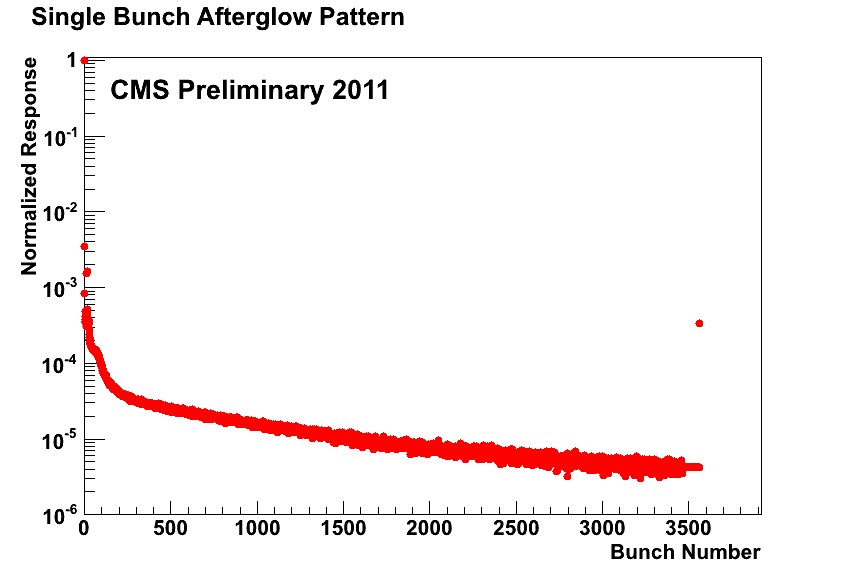
\includegraphics[width=0.5\columnwidth]{./SingleBunchAfterglow.png}
  \caption{Afterglow effect produced by a single colliding bunch.}
  \label{fig:LHC}
\end{figure}


Fig. 7 shows the afterglow noise induced by one colliding bunch. Since it is normalized to 1 at the first bin it means the first bin is the colliding bunch. The values at bins $>$ 1 are the cluster counts observed for bunches after the colliding bunch divided by the cluster counts observed by the colliding bunch. There are three parts to this distribution: \\

bin 1: colliding bunch \\

bin 2 (empty bunch): bunch after colliding bunch, noise observed is due to electronics signal on same pixels from colliding bunch. This is called Type 1. \\

bins $>$ 2 (empty bunches): noise observed is due to "albedo" which is material activated by the radiation of the collisions, it decays exponentially with time just like radioactive material. It produces secondary particles which create hits late in time. This is called Type 2.

\begin{figure}[H]
  \centering
  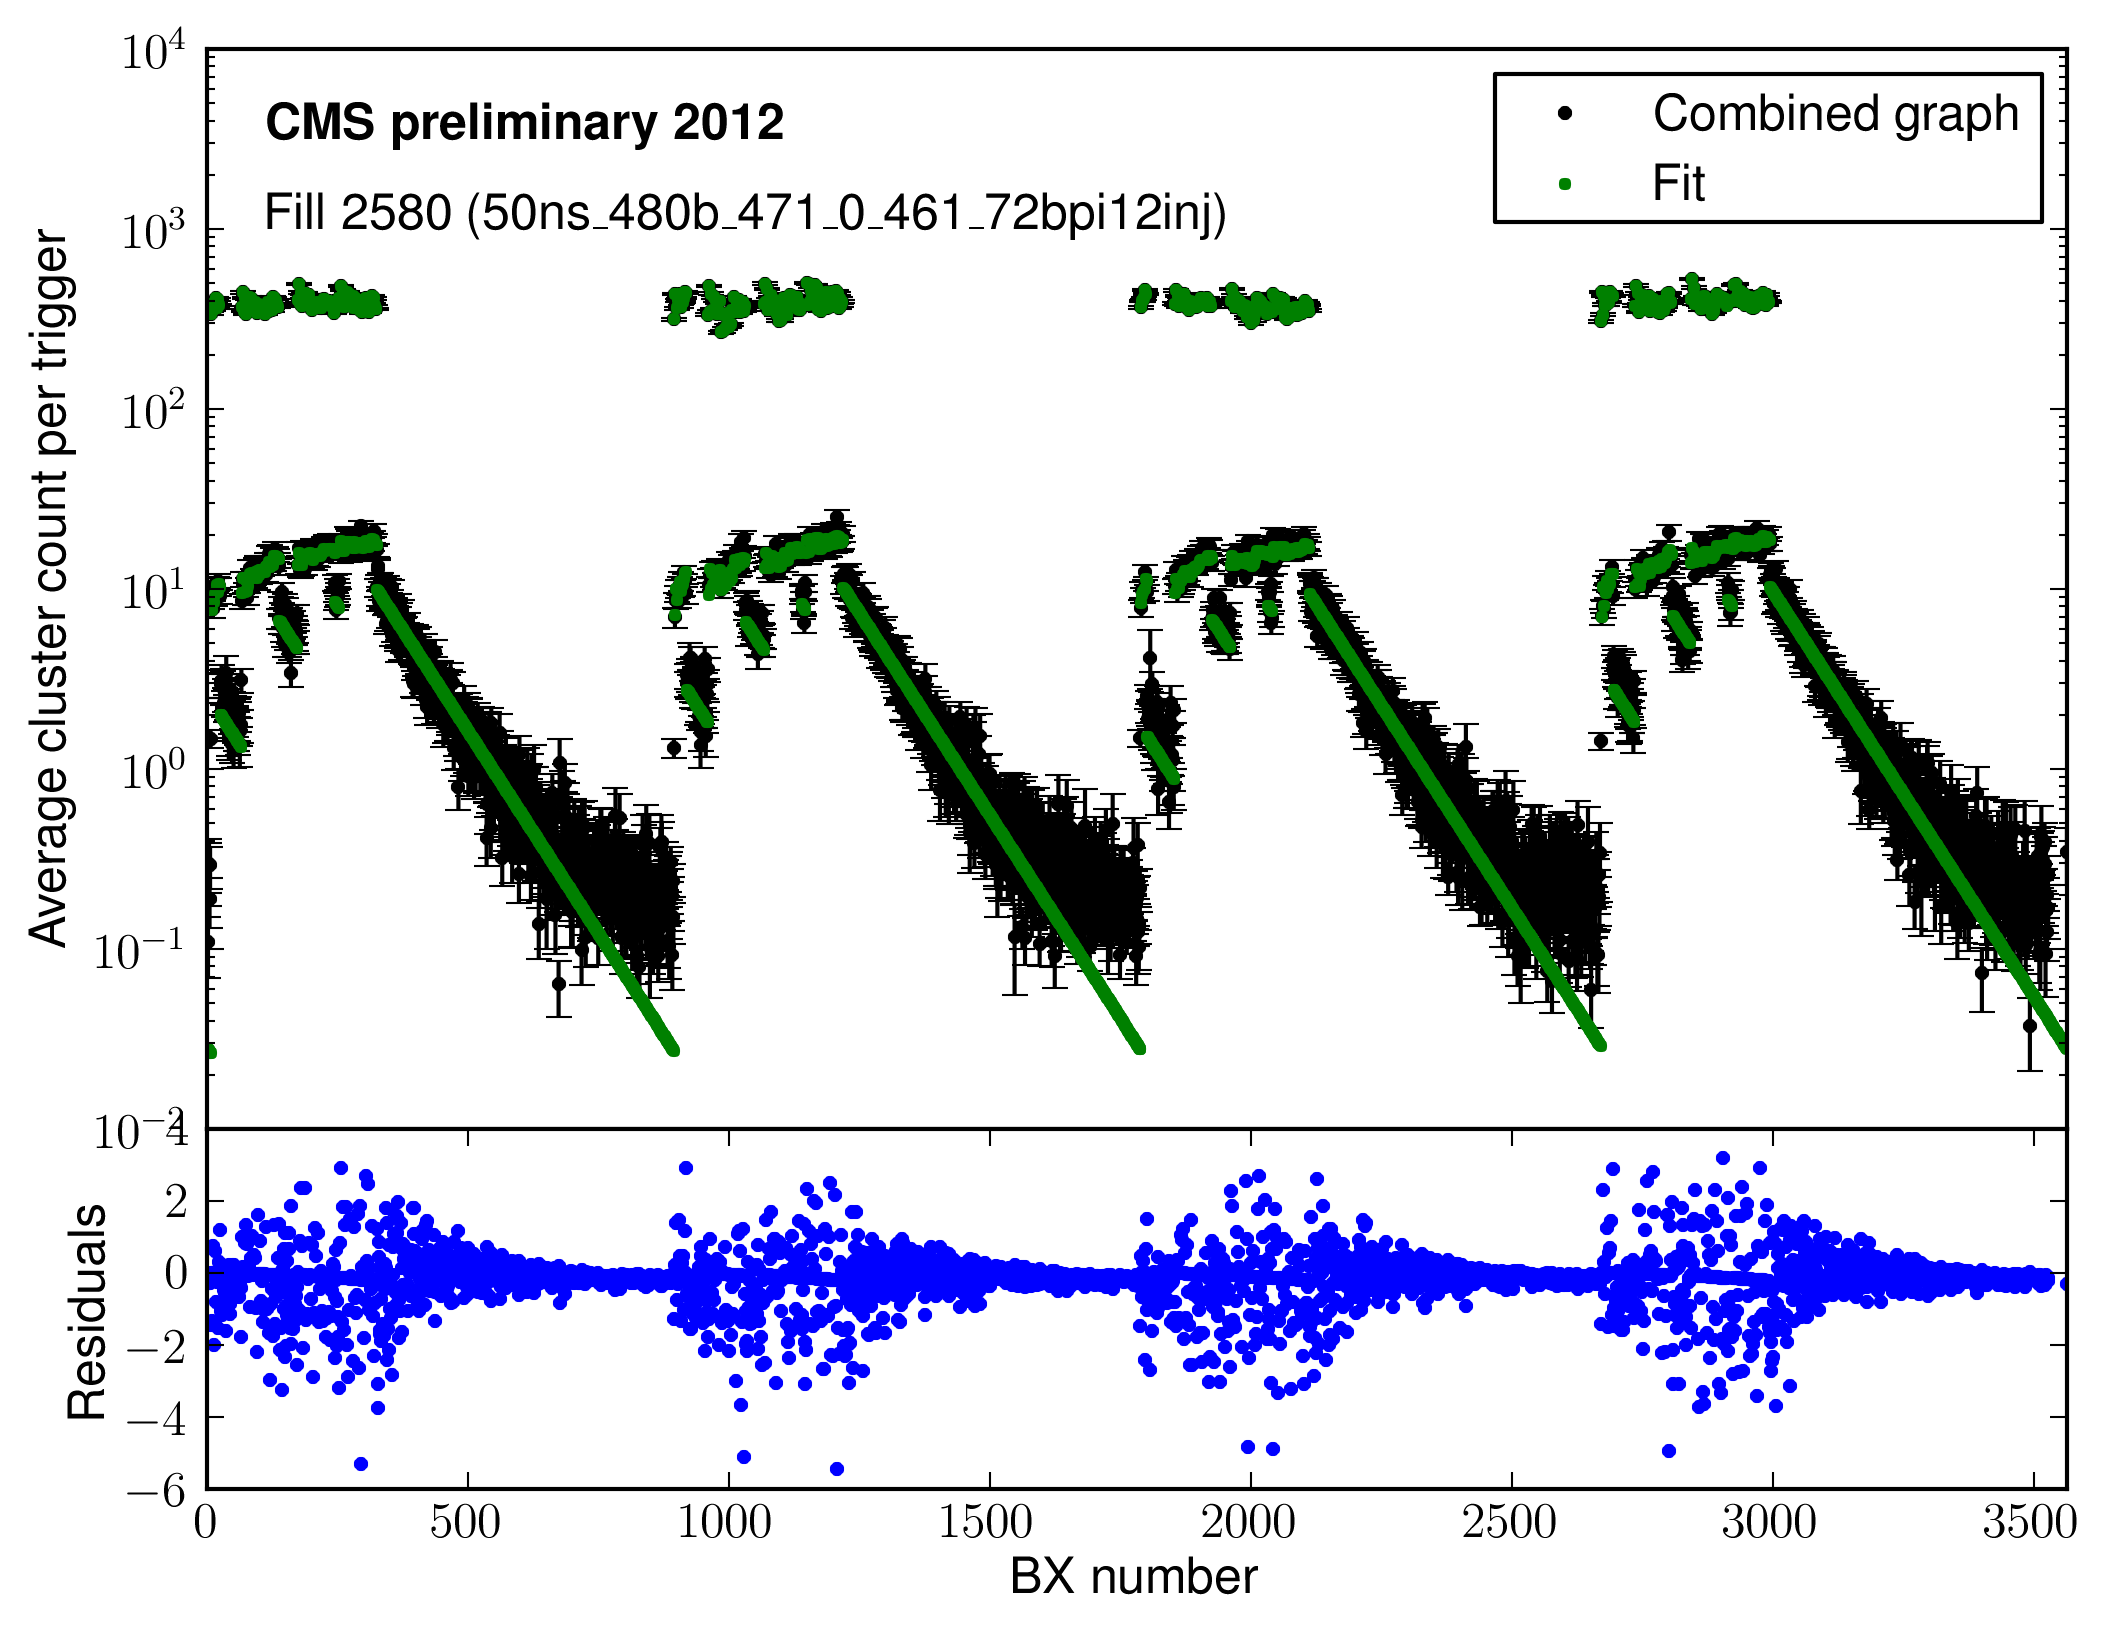
\includegraphics[width=0.5\columnwidth]{./afterglow.png}
  \caption{Results of the pixel afterglow 'deconvolution fit'}
  \label{fig:LHC}
\end{figure}


\begin{figure}[H]
  \centering
  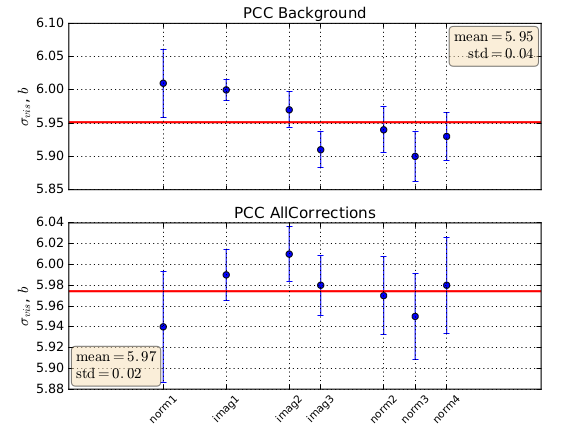
\includegraphics[width=0.6\columnwidth]{./PCC_background.png}
  \caption{ \onehalfspacing \cite{}.}
  \label{fig:CMS}
\end{figure}
